\documentclass[a4paper,10pt]{article}

\usepackage{amsfonts}
\usepackage{amssymb}
\usepackage{latexsym}
\usepackage{graphicx}
\usepackage{amssymb,amsmath}
\usepackage{listings}
\usepackage[titletoc]{appendix}
\usepackage{courier}
\usepackage[countmax]{subfloat}
\usepackage{here}

\linespread{1}

\hoffset -1in \topmargin 0mm \voffset 0mm \headheight 0mm
\headsep0mm
\oddsidemargin  20mm     %   Left margin on odd-numbered pages.
\evensidemargin 20mm     %   Left margin on even-numbered pages.
\textwidth   170mm       %   Width of text line.
\textheight  252mm

\makeatletter
\renewcommand\@openbib@code{%
     \advance\leftmargin  \z@ %\bibindent
      \itemindent \z@
     % Move bibitems close together
     \parsep -0.8ex
     }
\makeatother

\makeatletter
\renewcommand\section{\@startsection {section}{1}{\z@}%
                                   {-3.5ex \@plus -1ex \@minus -.2ex}%
                                   {2.3ex \@plus.2ex}%
                                   {\large\bfseries}}
\makeatother

\makeatletter
\renewcommand\subsection{\@startsection {subsection}{1}{\z@}%
                                   {-3.5ex \@plus -1ex \@minus -.2ex}%
                                   {2.3ex \@plus.2ex}%
                                   {\normalsize\bfseries}}
\makeatother

\begin{document}
\pagestyle{empty}

\begin{center}
{\bf \Large REVISITED BOX COUNTING TECHNIQUE IN BAYESIAN SENSE}
\end{center}

\smallskip
\begin{center} % David Blatsk\'{y}$^1$,
{\large David Blatsk\'{y}$^1$, Jarom\'{i}r Kukal$^1$, V\'{a}clav Hubata--Vacek$^1$}
\end{center}

\smallskip
\begin{center}
$^1$CTU in Prague, Faculty of Nuclear Sciences and Physical Engineering\\
Department of Software Engineering \\
B\v{r}ehov\'{a} 7, 115 19 Prague 1 \\
Czech Republic\\
blatsdav@fjfi.cvut.cz\\
 ~\\

\end{center}

\bigskip
\noindent Abstract: \textit{Fractal patterns appear in a wide variety of sources across nature. The unusual characteristic of fractals is that they entail non-integer dimension. The Box Counting method is one of the often used approach to estimate the fractal dimension of a signal. Thanks to the relationship between entropy and the fractal dimension, it is possible to employ entropy in estimating the fractal dimension. In this paper, we propose to utilize Bayesian estimate of Hartley entropy of a finite sample in fractal dimension estimation. This method was tested on artificial fractals generated by recursive expansion of appropriate matrices.}

\vspace*{10pt} \noindent Keywords: \textit{unbiased estimation, Hartley entropy, Shannon entropy, Box Counting}


\bigskip


\section {Introduction }
A fractal is an object whose so-called fractal dimension exceeds its topological dimension and its Hausdorff dimension is non-integer at the same time. The Box Counting method [\ref{bib:Box counting}] can be used for estimating the fractal dimension due to the relationship
\begin{equation} 
\label{eq:boxcount}
\ln{C(a)} = A - D_{0}\ln{a},
\end{equation}
where $a>0$ is a box size and $C(a)$ is a number of covering elements. Capacity dimension [\ref{bib:Capacity dimension}] $D_{0}$ is estimated as a slope of the line computed by the least square method. These estimates tend to be biased especially for small values of $a$. We propose to enhance the Box Counting method by Bayesian estimation of Hartley entropy $H_{0}$, which offers better estimate of capacity dimension $D_{0}$.

\section {Multinomial Distribution and Naive Entropy Estimates}

A multinomial distribution [\ref{bib:Multinomial Dirichlet}] model plays the main role in investigating of point set structures. Let $n \in \mathbb{N}$ be a number of distinguished events. Let $p_{j} > 0$ be a probability of the $j^{\text{th}}$ event for $j = 1,...,n$ satisfying $ \sum_{j=1}^{n} p_{j} =1$. Then the random variable $j$ has a multinomial distribution $\text{Mul}(p_{1},...,p_{n})$. After realization of multinomial distribution sample of size $N \in \mathbb{N}$, we can count the events and obtain $N_{j} \in \mathbb{N}_{0}$ as the number of $j^{\text{th}}$ event occurrences for $j=1,...,n$ satisfying $\sum_{j=1}^{n} N_{j} = N$. Therefore, we define the number of various events in a sample as $K = \sum_{N_{j}>0} 1 \le \text{min}(n,N)$. Revising Hartley [\ref{bib:Renyi}] and Shannon [\ref{bib:Renyi}] entropy definitions
\begin{equation} 
\label{eq:hnula}
H_{0}=\ln{n},
\end{equation} 
\begin{equation} 
\label{eq:hjedna}
H_{1}=-\sum_{j=1}^{n} p_{j}\ln{p_{j}},
\end{equation}   
we can perform a direct but naive estimation of them as
\begin{equation} 
\label{eq:hnulaap}
\hat{H}_{0,\mbox{\scriptsize{naive}}}=\ln{K},
\end{equation} 
\begin{equation} 
\label{eq:hjednaap}
\hat{H}_{1,\mbox{\scriptsize{naive}}}=-\sum_{N_{j}>0} \frac{N_{j}}{N}\ln{\frac{N_{j}}{N}}.
\end{equation}   
The main disadvantage of the naive estimates is their biasness. The random variable $K \in \{ 1,...,n \} $ is capped by $n$, which causes $\text{E}\hat{H}_{0,\mbox{\scriptsize{naive}}} = \text{E}\ln{K} < \text{E}\ln{n} = \ln{n} = H_{0}$. Hence, the naive estimate of Hartley entropy $\hat{H}_{0,\mbox{\scriptsize{naive}}}$ is negatively biased. On the other hand, the traditional Box Counting Technique is based on this estimate. There we plot the logarithm of the covering element number $C(a) \in \mathbb{N}$ against the logarithm of the covering element size $a > 0$ and then estimate their dependency in the linear form $\ln{C(a)} = A_{0} - \hat{D}_{0,\mbox{\scriptsize{naive}}}\ln{a}$. Recognizing equivalence $C(a) = K$ leads to $\ln{C(a)} = \ln{K} = \hat{H}_{0,\mbox{\scriptsize{naive}}}$ and then $\hat{H}_{0,\mbox{\scriptsize{naive}}} = A_{0} - \hat{D}_{0,\mbox{\scriptsize{naive}}}\ln{a}$. Defining $\hat{D}_{0,\mbox{\scriptsize{naive}}}$ as an estimate of capacity dimension and recognizing the occurrence of $\hat{H}_{0,\mbox{\scriptsize{naive}}}$ in the Box Counting procedure [\ref{bib:Box counting}], we are not surprised to be victims of the bias of Hartley entropy estimate.\\ 
\\*
A similar situation is the case of Shannon entropy estimation. There are several approaches how to decrease the bias of $\hat{H}_{1,\mbox{\scriptsize{naive}}}$ to be closer to a theoretical value of Shannon entropy $H_{1}$. Miller [\ref{bib:Harris}] modified the naive estimate $\hat{H}_{1,\mbox{\scriptsize{naive}}}$ using a first-order Taylor expansion resulting in
\begin{equation}
\label{eq:miller}
\hat{H}_{1,\mbox{\scriptsize{M}}}=\hat{H}_{1,\mbox{\scriptsize{naive}}} + \frac{K-1}{2N}.
\end{equation}
Lately, Harris [\ref{bib:Harris}] improved the formula to
\begin{equation}
\label{eq:harris1h}
\hat{H}_{1,\mbox{\scriptsize{H}}}=\hat{H}_{1,\mbox{\scriptsize{naive}}} + \frac{K-1}{2N} - \frac{1}{12N^2} \left( 1 - \sum_{p_{j}>0}\frac{1}{p_{j}} \right).
\end{equation}
Finally, we can estimate the capacity and information dimensions according to relation
\begin{equation} 
\label{eq:hjednaest}
\hat{H}_{d}=A_{d} - \hat{D}_{d} \ln{a},
\end{equation} 
where $\hat{H}_{d}$ is any estimate of $H_{d}$. Therefore, we can also estimate Hausdorff dimension $D_{\mbox{\scriptsize{H}}}$ using inequalities $D_{1} \le D_{\mbox{\scriptsize{H}}} \le D_{0}$ under the assumption that $\hat{D}_{1} \le D_{\mbox{\scriptsize{H}}} \le \hat{D}_{0}$ for any ``good'' estimates $\hat{D}_{0}$, $\hat{D}_{1}$ of capacity and information dimensions, respectively. The next section is oriented to Bayesian estimation of $H_{0}$ and $H_{1}$, which are essential for evaluating $\hat{D}_{0}$ and $\hat{D}_{1}$.

\section {Bayesian Estimation of Hartley Entropy}
We a suppose Dirichlet distribution of random vector $\vec{p} = (p_{1},...,p_{n})$ satisfying  $p_{j} \ge 0$, $\sum_{j=1}^{n} p_{j} = 1$, with $\alpha_j = ]alpha^{*} \ge 0$. Using properties of multinomial and its conjugate distribution --- the Dirichlet distributions, we can calculate probability $\text{p}(K|n,N)$ of the random variable $K \in \mathbb{N}$ for $K \le \min(n,N)$ as 
\begin{equation} 
\label{eq:pknn}
\mathrm{\hat{p}}(K \: | \: n,N) = \text{prob}\left(\sum_{N_{j} > 0}{1}=K \: \middle| \: n,\sum_{j=1}^{n}{N_{j}}=N\right) = {n \choose K} \frac{\Gamma({N+1}) \Gamma(n\alpha^{*})}{\Gamma(N+n\alpha^{*})} \sum_{\vec{N} \in \mathbb{D}_{K,N}} \prod_{j=1}^{K} \frac{ \Gamma(N_{j} + \alpha^{*})}{ \Gamma(N_j+1) \Gamma(\alpha^{*})}.
\end{equation}
Derivation of (\ref{eq:pknn}) is included in the Appendix \ref{subsec:app1}. When $N \ge K+2$, we can calculate 
\begin{equation} 
\label{eq:skn}
S_{K,N} = \sum_{n=K}^{\infty}{\mathrm{\hat{p}}\left(K \: \middle| \: n,N\right)}.
\end{equation}
When the number of events is constrained as $n \leq n_{\text{max}} $, we apply an alternative formula
\begin{equation} 
\label{eq:sknalt}
S_{K,N}^{*} = \sum_{n=K}^{n_{\text{max}}}{\mathrm{\hat{p}}\left(K \: \middle| \: n,N\right)}.
\end{equation}
Convergence of the infinite series (\ref{eq:skn}) is proved in the Appendix \ref{subsec:app2}. Having a knowledge of $K,N$ where $N \ge K+2$, we can calculate a Bayesian density
\begin{equation} 
\label{eq:pnkn}
\mathrm{\hat{p}}\left(n \: \middle| \: K,N \right) = \frac{\mathrm{\hat{p}}\left(K \: \middle| \: n,N\right)}{S_{K,N}},
\end{equation}
for $n \ge K$.
Therefore, Bayesian estimate of Hartley entropy is
\begin{equation} 
\label{eq:hnbayes}
\hat{H}_{0,\mbox{\scriptsize{Bayes}}} = \text{E}H_{0}  = \sum_{n=K}^{\infty}{\mathrm{\hat{p}}\left(n \: \middle| \: K,N\right)\ln{n}} = \sum_{n=K}^{\infty} \frac{\mathrm{\hat{p}}\left(K \: \middle| \: n,N\right)\ln{n}}{S_{K,N}} =  \frac{ \sum_{n=K}^{\infty} \mathrm{\hat{p}}\left(K \: \middle| \: n,N\right)\ln{n}}{\sum_{n=K}^{\infty} \mathrm{\hat{p}}\left(K \: \middle| \: n,N\right)} > \ln{K}
\end{equation}
which is also a convergent sum. Substituting $n=K+j$ we gain equivalent formula
\begin{equation} 
\label{eq:hnbayesb}
\hat{H}_{0,\mbox{\scriptsize{Bayes}}} = \frac{\sum_{j=0}^{\infty}{b_{j}\ln{(K+j)}}}{\sum_{j=0}^{\infty}{b_j}}
\end{equation}
where $b_{j}= {K+j \choose j} \frac{\mathrm{B}\left( (K+j)\alpha^{*}, N \right)}{\mathrm{B}\left( K\alpha^{*}, N \right)}$. Particular coeficients $b_{j}$ can also be generated by recursive formula
\begin{equation}
\label{eq:breform}
\begin{split}
& b_{0} = 1 \\
& b_{j} = \frac{(K+j)}{j} \frac{\Gamma{((K+j)\alpha^{*})}}{\Gamma{((K+j)\alpha^{*}-\alpha^{*})}}\frac{\Gamma{(N+(K+j)\alpha^{*} -\alpha^{*})}}{\Gamma({N+(K+j)\alpha^{*})}} b_{j-1}.
\end{split}
\end{equation}
Asymptotic properties of the Bayesian estimate for $N \rightarrow +\infty$ can be investigated via limits
\begin{equation} 
\label{eq:lim}
\begin{split}
\lim_{N \rightarrow +\infty} & {\hat{H}_{0,\mbox{\scriptsize{Bayes}}}} = \ln{K}, \\
\lim_{N \rightarrow +\infty} & {(\hat{H}_{0,\mbox{\scriptsize{Bayes}}}-\ln{K})N} = K(K+1)\ln(1+1/K), \\
\lim_{N \rightarrow +\infty} & {\left(\hat{H}_{0,\mbox{\scriptsize{Bayes}}}-\ln{K}-\frac{K(K+1)\ln(1+1/K)}{N}\right)N^2} = \\
& \frac{1}{2}\left(K(K+2)(K+1)\left(\ln(K+2)-\ln(K)-2K\ln(K+1)+K\ln(K+2)+K\ln(K)\right)\right),
\end{split}
\end{equation}
Therefore
\begin{equation} 
\label{eq:hroz}
\begin{split}
\hat{H}_{0,\mbox{\scriptsize{Bayes}}} \approx & \ln{K} + \frac{K(K+1)\ln(1+1/K)}{N} + \\ 
& \frac{\left(K(K+2)(K+1)\left(\ln(K+2)-\ln(K)-2K\ln(K+1)+K\ln(K+2)+K\ln(K)\right)\right)}{2N^2}
\end{split}
\end{equation}
When $K$ is also large, we can roughly approximate Hartley entropy as
\begin{equation} 
\label{eq:hartapp}
\hat{H}_{0,\mbox{\scriptsize{Bayes}}} \approx \ln{K} + \frac{K+1}{N}
\end{equation}
which is very similar to Miller correction (\ref{eq:miller}) in the case of Shannon entropy estimation. Meanwhile formula (\ref{eq:hnbayes}) represents Bayesian estimate of $H_{0}$, formulas (\ref{eq:hnulaap}), (\ref{eq:hartapp}), and (\ref{eq:hroz}) are approximations of zero, first, and second order. \\
\\*
Formula (\ref{eq:hnbayesb}) can be also expanded to the form
\begin{equation} 
\label{eq:hnbayesbexp}
\hat{H}_{0,\mbox{\scriptsize{Bayes}}} = \ln{K} + \sum_{j=1}^{\infty} \frac{1}{j} \varphi(K)\left(\frac{K}{N}\right)^{j}
\end{equation}
where $\varphi(K)>1$ for all $K \in \mathbb{N}$ and $\lim_{K \rightarrow \infty} \varphi(K) = 1$. Therefore, we obtain lower estimate
\begin{equation}
\label{eq:hnbayesbexplow}
\hat{H}_{0,\mbox{\scriptsize{Bayes}}} > \ln{K} + \sum_{j=1}^{\infty} \frac{1}{j} \left(\frac{K}{N}\right)^{j} = \ln{K} - \ln(1 - \frac{K}{N}) = H_{0,\mbox{\scriptsize{low}}}
\end{equation}
which exists for $K < N$.

\section {Bayesian Estimation of Shannon Entropy}
In the case when the number of events $n$ is known, we perform Bayesian estimation of Shannon entropy for arbitrary $\alpha_j = \alpha^{*} > 0$ as
\begin{equation} 
 -\sum_{i=1}^M \frac{\Gamma(N+\alpha)}{\Gamma(n_i+\alpha_i)} \frac{\Gamma(n_i+\alpha_i+1)}{\Gamma(N+\alpha+ 1)}\left(\psi^{(0)}(n_i+\alpha_i+1) -\psi^{(0)}(N+\alpha+ 1) \right) 
\end{equation}
\begin{equation} 
\label{eq:hjednan}
\begin{split}
\hat{H}_{1,\mathrm{n}} & = \text{E}H_{1}(K=n) \\ & = -\sum_{j=1}^{n} \left( \frac{N_{j}+\alpha^*}{N+n\alpha^*} \left( \psi(N_{j}+\alpha^*+1) - \psi(N+n\alpha^*+1) \right) \right),
\end{split}
\end{equation}
where $\psi$ is digamma function. However, when the number of events $n$ is unknown, we can use $K$ as a lower estimate of $n$ and perform the final Bayesian estimation as
\begin{equation} 
\label{eq:hjednab}
\hat{H}_{1,\mathrm{Bayes}} = \sum_{n=K}^{\infty}{\text{p}\left(n \: \middle| \:K,N \right)\hat{H}_{1,\mathrm{n}}},
\end{equation}
which is also a convergent sum for $N \ge K+2$. \\
\\*
Substituting $n=K+j$, we obtain an adequate formula
\begin{equation} 
\label{eq:hjbb}
\hat{H}_{1,\mathrm{Bayes}} = \frac{\sum_{j=0}^{\infty}b_{j}\hat{H}_{1,K+j}}{\sum_{j=0}^{\infty}b_{j}}.
\end{equation}
Unfortunately, asymptotic expansion of (\ref{eq:hjbb}) depends on individual frequencies $N_{j}$. But $\hat{H}_{1,n} \leq \ln{n}$, hence $\hat{H}_{1,K+j} \leq \ln{K+j}$, which implies the convergence of~$\sum_{j=0}^{\infty}b_{j}\hat{H}_{1,K+j}$ based on majority rule and (\ref{eq:hnbayesb}).

\section {Revisited Box Counting Method}
Let $\mathbb{F} \subset \mathbb{R}^{m}$ be a set of $N$ points placed into $m$-dimensional rectangular grid of element size $a > 0$. Let $\hat{H}_{0,\mathrm{Bayes}}$ be an unbiased estimate of Hartley entropy $H_{0}$. Fitting the linear model
\begin{equation} 
\label{eq:hlinmod}
\hat{H}_{0,\mathrm{Bayes}} = A - \hat{D}_{0}\ln{a}
\end{equation}
via the method of least squares is called Revisited Box Counting.\\
\\*
Revisited Box Counting can be modified by %:
%\begin{itemize}
%\item 
using $\hat{H}_{1,\mathrm{Bayes}}$ instead of $\hat{H}_{0,\mathrm{Bayes}}$ which comes to estimation of information dimension [\ref{bib:Information dimension}] according to
\begin{equation} 
\label{eq:inform}
\hat{H}_{1,\mathrm{Bayes}} = A - \hat{D}_{1}\ln{a}.
\end{equation}
%\item using non-trivial approximations of $\hat{H}_{0,\mbox{\scriptsize{Bayes}}}$, namely: $\hat{H}_{0,1}, \hat{H}_{0,2}, \hat{H}_{0,\mbox{\scriptsize{low}}}$ instead of $\hat{H}_{0,\mbox{\scriptsize{Bayes}}}$
%\end{itemize}
%Remark: \\
%Using of $\hat{H}_{0,0} \equiv \hat{H}_{0,\mbox{\scriptsize{naive}}}$ instead of $\hat{H}_{0,\mbox{\scriptsize{Bayes}}}$ comes back to traditional Box Counting.

\section {Experimental Part }

The Revisited Box Counting technique will be tested on models of deterministic self-similar 2D fractal sets. They are generated by recursive expansion of binary matrix $\mathbb{G}_{u,v} \in \{ 0, 1 \}^{v \times v} $, where $u$ a is the number of non-zero elements (units), $v>1$ is a matrix dimension, and $v<u<v^2$. \\
\\*
Recursive expansion of $\mathbb{G}_{u,v}$ generates a binary matrix which represents fractal set $\mathbb{F}_{u,v}$ of a similarity dimension $D_{\text{S}} = D_{\text{H}} = D_{0} = D_{1} = \frac{\log{u}}{\log{v}}$. Depth $h$ of recursion depends on $v$ and should be appropriate to computer memory size.\\
\\*
Four testing sets $\mathbb{F}_{3,2}$, $\mathbb{F}_{4,3}$, $\mathbb{F}_{5,3}$, $\mathbb{F}_{8,3}$ were generated by matrices:
\begin{itemize}
\item 

$\mathbb{G}_{3,2} = \begin{bmatrix}
1 & 1 \\
1 & 0 
\end{bmatrix}$ for $h=11$, $\text{dim}(\mathbb{F}_{3,2}) = \frac{\log{3}}{\log{2}} = 1.5850,$

\item 

$\mathbb{G}_{4,3} = \begin{bmatrix}
0 & 1 & 0 \\
1 & 0 & 1 \\
0 & 1 & 0
\end{bmatrix}$ for $h=7$, $\text{dim}(\mathbb{F}_{4,3}) = \frac{\log{4}}{\log{3}} = 1.2619,$

\item 

$\mathbb{G}_{5,3} = \begin{bmatrix}
0 & 1 & 0 \\
1 & 1 & 1 \\
0 & 1 & 0
\end{bmatrix}$ for $h=7$, $\text{dim}(\mathbb{F}_{5,3}) = \frac{\log{5}}{\log{3}} = 1.4650,$

\item 

$\mathbb{G}_{8,3} = \begin{bmatrix}
1 & 1 & 1 \\
1 & 0 & 1 \\
1 & 1 & 1
\end{bmatrix}$ for $h=7$, $\text{dim}(\mathbb{F}_{8,3}) = \frac{\log{8}}{\log{3}} = 1.8928.$
\end{itemize}
Sets $\mathbb{G}_{3,2}$ and $\mathbb{G}_{8,3}$ correspond to Sierpinski gasket and carpet respectively. \\
\\*
At first, adequate point sets of given depth $h$ were generated. Then, they were randomly rotated around the origin, and finally they were randomly shifted. Afterwards, a grid of size $a$ was put on the data points and entropy estimates were calculated. Due to physical interpretation of entropy, the estimates were averaged over 10 realizations and mean values of entropy were calculated. \\
\\*
Various estimates of Hartley entropy for the grid of size $a=5,7,10,15,...,150,200$ are depicted in Fig \ref{fig:frac}. Hartley entropy estimates are similar to each other except for under-biased naive estimate. Estimates $H_{0,\mbox{\scriptsize{BAYES}}}$ and $H_{0,\mbox{\scriptsize{low}}}$ are very similar in these four cases. Corresponding estimates of Shannon entropy are depicted in Fig. \ref{fig:fracshan} in the same range. \\
\\*
As seen in Fig. \ref{fig:frac} and \ref{fig:fracshan}, too small grid size $a \leq 20$ comes to underestimation of $\hat{H}_{0,\mbox{\scriptsize{naive}}}, \hat{H}_{1,\mbox{\scriptsize{naive}}}$, but the other estimates are unfortunately overestimated. Therefore, Revisited Box Counting was applied in the range $30 \leq a \leq 100$.\\
\\*
Using the least square method we obtained various estimates of $D_{0}$ and $D_{1}$ and got a chance to compare them with theoretical values of similarity dimension. The results of estimation are collected in Tabs. \ref{tab:est1} - \ref{tab:est4s}, where $\text{E}D$ is point estimate of a given dimension, $s_{D}$ is its standard deviation, and $p_{\text{value}}$ is probability from t-test of hypothesis
\begin{equation} 
\label{eq:hypo}
\text{H}_{0} : \text{E}D = D_{\text{S}}.
\end{equation}

\section {Conclusion}
In this paper we derived the Bayesian estimator $\hat{H}_{0,\mbox{\scriptsize{Bayes}}}$ of Hartley entropy for a general value of the parameter $\alpha^*$. As shown, similar approach can also be used to estimate Shannon entropy $\hat{H}_{1,\mbox{\scriptsize{Bayes}}}$. These both can result in less biased estimates of the appropriate entropy when used with proper $\alpha^*$ and the grid size $a$. According to the relation between fractal (information) dimension and Hartley (Shannon) entropy, we estimated dimensions from experimental data. The results turned out to be significantly more accurate than those estimated naively without a priory information.


\vspace*{10pt} \noindent {\bf Acknowledgement:} The authors acknowledge the funding from the CTU in Prague, \\ Grant SGS14/208/OHK4/3T/14.

\begin{thebibliography}{99}
\vskip12pt
\bibitem{Harris}\label{bib:Harris} Harris, B., \textit{The statistical estimation of entropy in the non-parametric case}. MRC Technical Summary Report, 1975. 
\bibitem{Wendel}\label{bib:Wendel} Wendel, J., \textit{Note on the gamma function}. Amer. Math. Monthly, 55(1948), 563-564.
\bibitem{Renyi}\label{bib:Renyi} Renyi, A., \textit{On measures of entropy and information}. In Proc. Fourth Berkeley Symp. Math. Stat. Prob., 1960, volume 1, page 547, Berkeley, 1961. University of California Press.
\bibitem{Capacity_dimension}\label{bib:Capacity dimension} Baker, G. L. and Gollub, J. B. \textit{Chaotic Dynamics: An Introduction, 2nd ed.} Cambridge, England: Cambridge University Press, 1996.
\bibitem{Information_dimension}\label{bib:Information dimension} Ott, E. \textit{Chaos in Dynamical Systems.} New York: Cambridge University Press, p. 79, 1993.
\bibitem{Box_counting}\label{bib:Box counting} Mandelbrot, B. B. \textit{The Fractal Geometry of Nature}. W.H. Freeman and Company, 1982.
\bibitem{Multinomial_Dirichlet}\label{bib:Multinomial Dirichlet} S. Kotz, N. Balakrishnan, and N. L. Johnson. \textit{Continuous Multivariate Distributions. Volume 1: Models and Applications.} New York: Wiley, 2000. ISBN 0-471-18387-3.
\bibitem{Raabe}\label{bib:Raabe} Bromwich, T. J. I'A. and MacRobert, T. M. \textit{An Introduction to the Theory of Infinite Series, 3rd ed.} New York: Chelsea, p. 39, 1991.

%
\begin{figure}[H]
\centering
\begin{tabular}{cc}
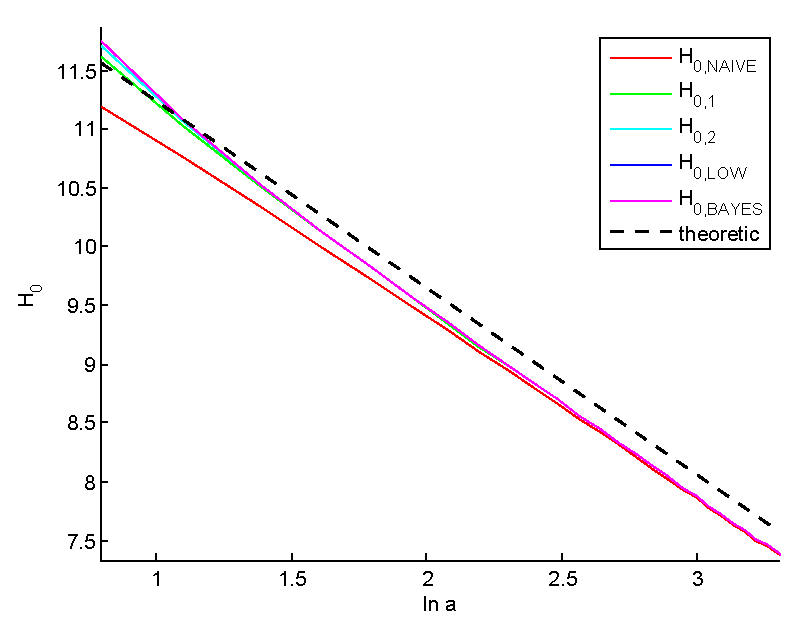
\includegraphics[width=0.4\textwidth]{images5/frac32i.pdf} &
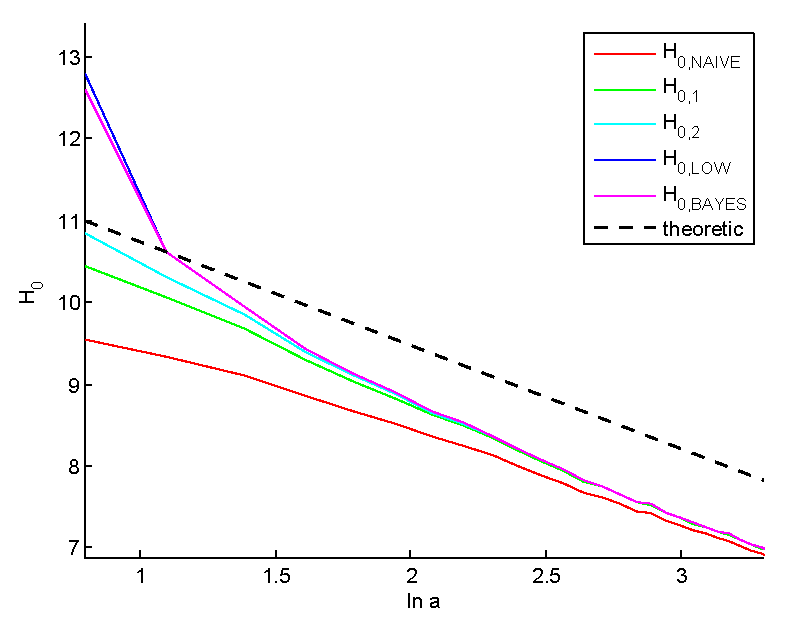
\includegraphics[width=0.4\textwidth]{images5/frac43i.pdf} \\
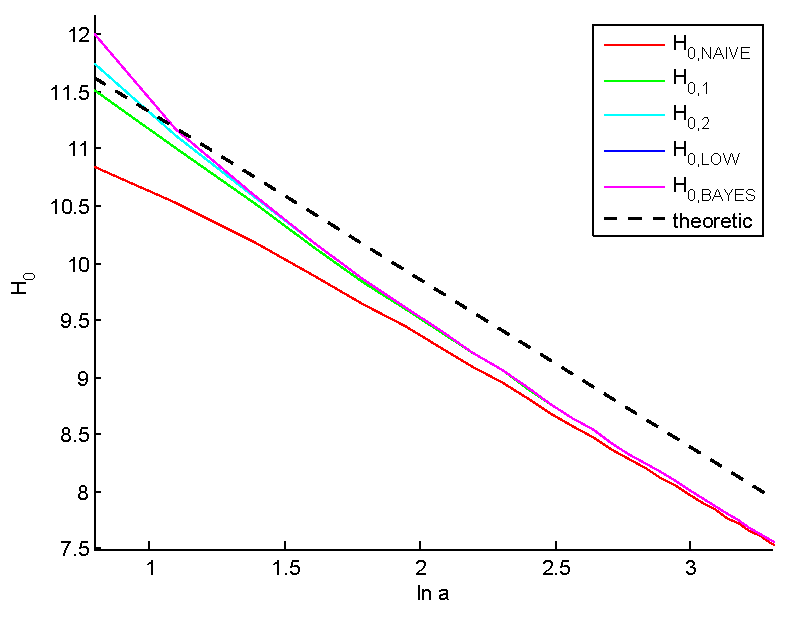
\includegraphics[width=0.4\textwidth]{images5/frac53i.pdf} &
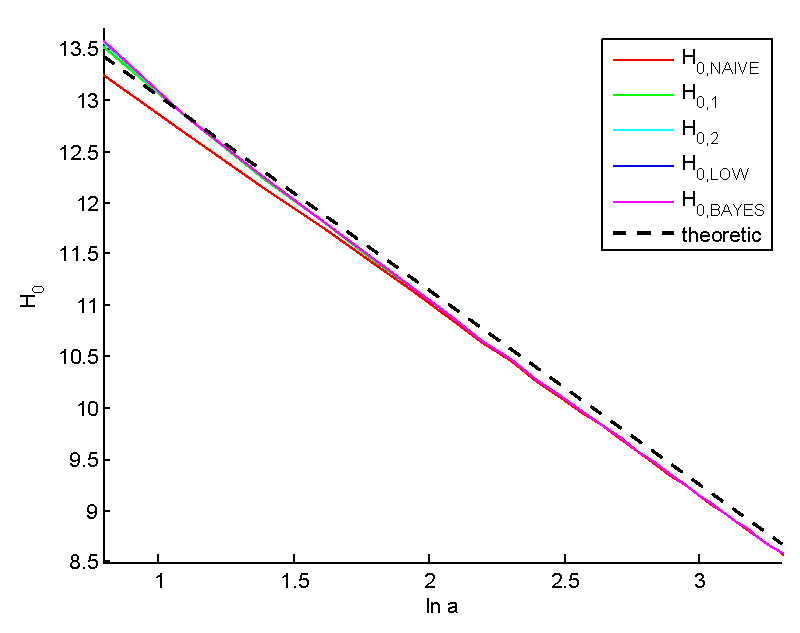
\includegraphics[width=0.4\textwidth]{images5/frac83i.pdf}
\end{tabular}
\caption{Hartley entropy estimates: $F_{32}$ (top left), $F_{43}$ (top right), $F_{53}$ (bottom left), $F_{83}$ (bottom right) }
\label{fig:frac}
\end{figure}


\begin{figure}[H]
\centering
\begin{tabular}{cc}
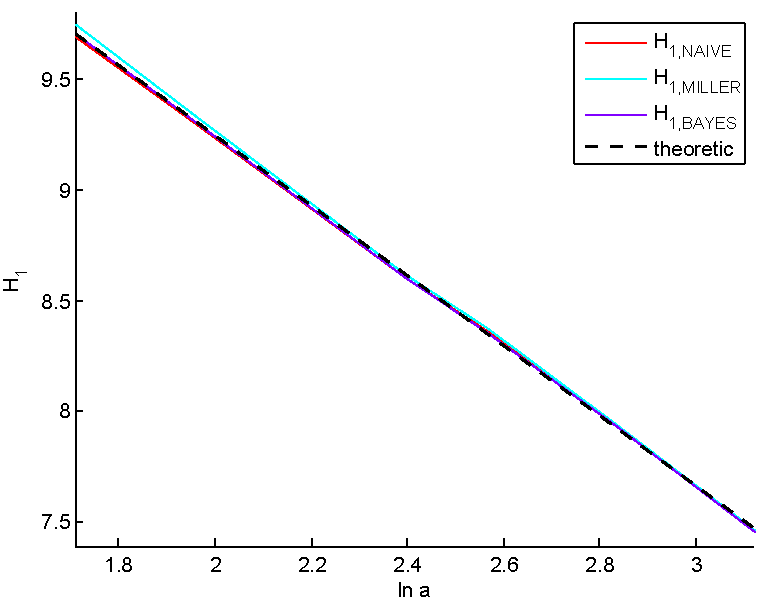
\includegraphics[width=0.4\textwidth]{images4/frac32si.pdf} &
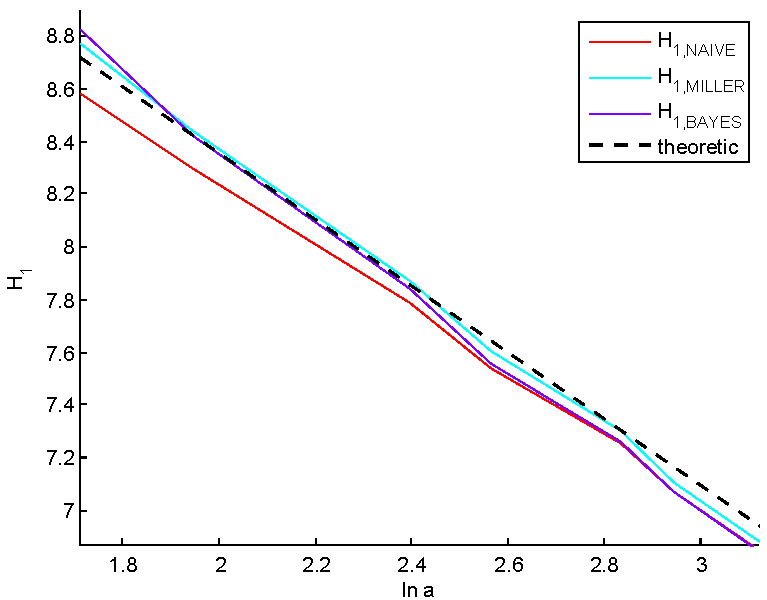
\includegraphics[width=0.4\textwidth]{images4/frac43si.pdf} \\
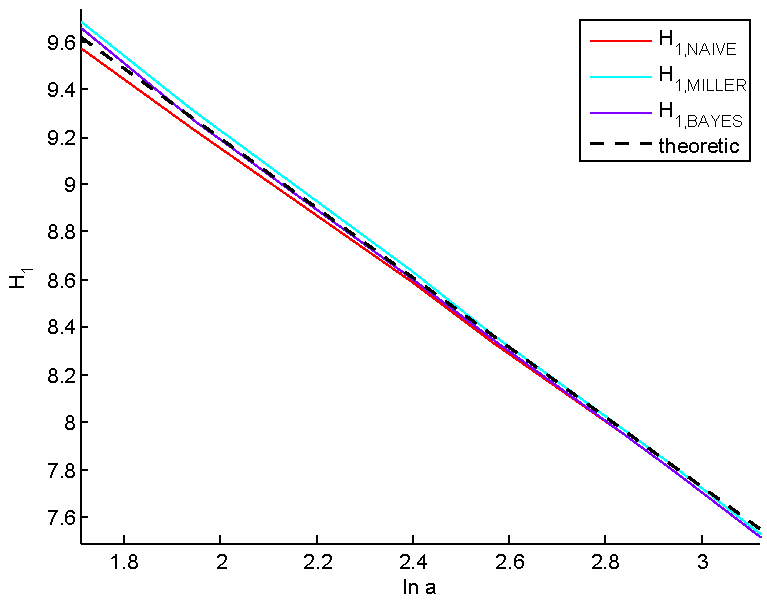
\includegraphics[width=0.4\textwidth]{images4/frac53si.pdf} &
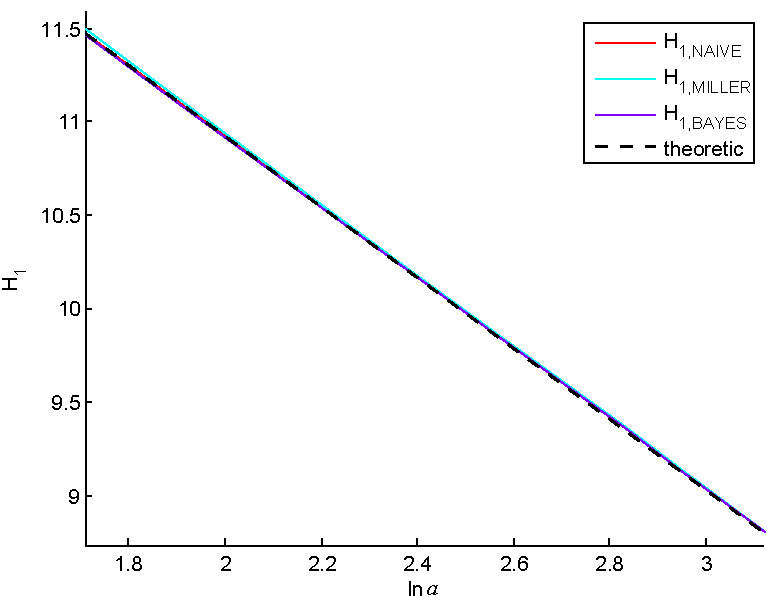
\includegraphics[width=0.4\textwidth]{images4/frac83si.pdf}
\end{tabular}
\caption{Shannon entropy estimates: $F_{32}$ (top left), $F_{43}$ (top right), $F_{53}$ (bottom left), $F_{83}$ (bottom right) }
\label{fig:fracshan}
\end{figure}
%
%\begin{table}[H] 
\begin{center}
\caption{Dimension estimates for $\mathbb{F}_{3,2}$}
\label{tab:est1}
\begin{tabular}{|l|l|l|l|}
\hline
 estimate & \multicolumn{3}{c|}{$\mathbb{F}_{3,2}$} \\
\hline
 & $\hat{D}$ & $s_{D}$ & $z_{\mbox{\scriptsize{score}}}$ \\
\hline 
$ H_{0,\mbox{\scriptsize{naive}}} $ & 1.5714 & 0.0052 & -2.6384 \\ 
\hline 
$ H_{0,1} $ & 1.5765 & 0.0051 & -1.6604 \\ 
\hline 
$ H_{0,2} $ & 1.5765 & 0.0051 & -1.6565 \\ 
\hline 
$ H_{0,\mbox{\scriptsize{low}}} $ & 1.5765 & 0.0051 & -1.6565 \\ 
\hline 
$ H_{0,\mbox{\scriptsize{Bayes}}} $ & 1.5765 & 0.0051 & -1.6565 \\ 
\hline 
\end{tabular}
\end{center}
\end{table} 

\begin{table}[H] 
\begin{center}
\caption{Dimension estimates for $\mathbb{F}_{4,3}$}
\label{tab:est2}
\begin{tabular}{|l|l|l|l|}
\hline
 estimate & \multicolumn{3}{c|}{$\mathbb{F}_{4,3}$} \\
\hline
 & $\hat{D}$ & $s_{D}$ & $z_{\mbox{\scriptsize{score}}}$ \\
\hline 
$ H_{0,\mbox{\scriptsize{naive}}} $ & 1.2233 & 0.0136 & -2.8259 \\ 
\hline 
$ H_{0,1} $ & 1.2565 & 0.0135 & -0.3963 \\ 
\hline 
$ H_{0,2} $ & 1.2575 & 0.0135 & -0.3202 \\ 
\hline 
$ H_{0,\mbox{\scriptsize{low}}} $ & 1.2576 & 0.0135 & -0.3177 \\ 
\hline 
$ H_{0,\mbox{\scriptsize{Bayes}}} $ & 1.2576 & 0.0135 & -0.3175 \\ 
\hline  
\end{tabular}
\end{center}
\end{table} 

\begin{table}[H] 
\begin{center}
\caption{Dimension estimates for $\mathbb{F}_{5,3}$}
\label{tab:est3}
\begin{tabular}{|l|l|l|l|}
\hline
 estimate & \multicolumn{3}{c|}{$\mathbb{F}_{5,3}$} \\
\hline
 & $\hat{D}$ & $s_{D}$ & $z_{\mbox{\scriptsize{score}}}$ \\
\hline 
$ H_{0,\mbox{\scriptsize{naive}}}  $ & 1.4484 & 0.0082 & -2.0304 \\ 
\hline 
$ H_{0,1} $ & 1.4616 & 0.0081 & -0.4159 \\ 
\hline 
$ H_{0,2} $ & 1.4617 & 0.0081 & -0.3983 \\ 
\hline 
$ H_{0,\mbox{\scriptsize{low}}} $ & 1.4617 & 0.0081 & -0.3981 \\ 
\hline 
$ H_{0,\mbox{\scriptsize{Bayes}}} $ & 1.4617 & 0.0081 & -0.3981 \\ 
\hline 
\end{tabular}
\end{center}
\end{table}

\begin{table}[H] 
\begin{center}
\caption{Dimension estimates for $\mathbb{F}_{8,3}$}
\label{tab:est4}
\begin{tabular}{|l|l|l|l|}
\hline
 estimate & \multicolumn{3}{c|}{$\mathbb{F}_{8,3}$} \\
\hline
 & $\hat{D}$ & $s_{D}$ & $z_{\mbox{\scriptsize{score}}}$ \\
\hline
$ H_{0,\mbox{\scriptsize{naive}}} $ & 1.8398 & 0.0040 & -13.0862 \\ 
\hline 
$ H_{0,1} $ & 1.8413 & 0.0042 & -12.4030 \\ 
\hline 
$ H_{0,2} $ & 1.8413 & 0.0042 & -12.4020 \\ 
\hline 
$ H_{0,\mbox{\scriptsize{low}}} $ & 1.8413 & 0.0042 & -12.4020 \\ 
\hline 
$ H_{0,\mbox{\scriptsize{Bayes}}} $ & 1.8413 & 0.0042 & -12.4020 \\ 
\hline 
\end{tabular}
\end{center}
\end{table}







\begin{table}[H] 
\begin{center}
\caption{Dimension estimates for $\mathbb{F}_{3,2}$}
\label{tab:est1s}
\begin{tabular}{|l|l|l|l|}
\hline
 estimate & \multicolumn{3}{c|}{$\mathbb{F}_{3,2}$} \\
\hline
 & $\hat{D}$ & $s_{D}$ & $z_{\mbox{\scriptsize{score}}}$ \\
\hline
$ H_{1,\mbox{\scriptsize{naive}}} $ & 1.5797 & 0.0030 & -1.7182 \\ 
\hline 
$ H_{1,\mbox{\scriptsize{Miller}}} $ & 1.5823 & 0.0031 & -0.8626 \\ 
\hline 
$ H_{1,\mbox{\scriptsize{Bayes}}} $ & 1.5797 & 0.0030 & -1.7155 \\ 
\hline 
\end{tabular}
\end{center}
\end{table}

\begin{table}[H] 
\begin{center}
\caption{Dimension estimates for $\mathbb{F}_{4,3}$}
\label{tab:est2s}
\begin{tabular}{|l|l|l|l|}
\hline
 estimate & \multicolumn{3}{c|}{$\mathbb{F}_{4,3}$} \\
\hline
 & $\hat{D}$ & $s_{D}$ & $z_{\mbox{\scriptsize{score}}}$ \\
\hline 
$ H_{1,\mbox{\scriptsize{naive}}} $ & 1.2698 & 0.0072 & 1.1093 \\ 
\hline 
$ H_{1,\mbox{\scriptsize{Miller}}} $ & 1.2866 & 0.0069 & 3.5709 \\ 
\hline 
$ H_{1,\mbox{\scriptsize{Bayes}}} $ & 1.2763 & 0.0071 & 2.0192 \\ 
\hline 
\end{tabular}
\end{center}
\end{table}

\begin{table}[H] 
\begin{center}
\caption{Dimension estimates for $\mathbb{F}_{5,3}$}
\label{tab:est3s}
\begin{tabular}{|l|l|l|l|}
\hline
 estimate & \multicolumn{3}{c|}{$\mathbb{F}_{5,3}$} \\
\hline
 & $\hat{D}$ & $s_{D}$ & $z_{\mbox{\scriptsize{score}}}$ \\
\hline 
$ H_{1,\mbox{\scriptsize{naive}}} $ & 1.4691 & 0.0046 & 0.9019 \\ 
\hline 
$ H_{1,\mbox{\scriptsize{Miller}}} $ & 1.4757 & 0.0048 & 2.2218 \\ 
\hline 
$ H_{1,\mbox{\scriptsize{Bayes}}} $ & 1.4717 & 0.0046 & 1.4442 \\ 
\hline 
\end{tabular}
\end{center}
\end{table}

\begin{table}[H] 
\begin{center}
\caption{Dimension estimates for $\mathbb{F}_{8,3}$}
\label{tab:est4s}
\begin{tabular}{|l|l|l|l|}
\hline
 estimate & \multicolumn{3}{c|}{$\mathbb{F}_{8,3}$} \\
\hline
 & $\hat{D}$ & $s_{D}$ & $z_{\mbox{\scriptsize{score}}}$ \\
\hline
$ H_{1,\mbox{\scriptsize{naive}}}  $ & 1.8641 & 0.0013 & -22.3767 \\ 
\hline 
$ H_{1,\mbox{\scriptsize{Miller}}} $ & 1.8648 & 0.0013 & -21.1850 \\ 
\hline 
$ H_{1,\mbox{\scriptsize{Bayes}}} $ & 1.8638 & 0.0013 & -22.9511 \\ 
\hline 
\end{tabular}
\end{center}
\end{table}



\newpage

\end{thebibliography}
\begin{appendices}

\section {Appendix}


\subsection {Derivation of $\hat{\mathrm{p}}(K|n,N)$ in (\ref{eq:pknn})}
\label{subsec:app1}
Let $\mathbb{Q}_{n} = \{ \vec{q} \in (\mathbb{R}_{0}^{+})^{n} | \sum_{j=1}^{n}q_{j} = 1 \}$ be a support set of a Dirichlet-distributed random variable $\vec{p} \in \mathbb{Q}_{n}$ with parameters $\alpha_j$, for $j = 1,...,n$. The conditional probability of an~integer $K$ satisfying $1 \le K \le \min(n,N)$ is 
\begin{equation} 
\label{eq:probpkn}
\text{p}(K \: | \: n,N) = \text{prob}\left(\sum_{N_{j}>0} 1 = K \: \middle| \: n, \sum_{j=1}^{n}N_{j} = N\right).
\end{equation}
The vector of $N_{j}$ can be reorganized to begin with positive values:
\begin{equation} 
\label{eq:probbinom}
\text{p}(K \: | \: n,N) = \binom{n}{K}\text{prob}\left( \forall j=1,...,n : N_{j} > 0 \Leftrightarrow j \le K \: \middle| \: n, \sum_{j=1}^{K}N_{j}=N\right).
\end{equation}
Let $\mathbb{D}_{K,N} = \{ \vec{x} \in \mathbb{N}^K | \sum_{j=1}^{K}x_{j} = N \}$ be the domain of $\vec{N} = (N_{1},...,N_{K}) \in \mathbb{D}_{K,N}$. Using the mean value of a~multinomial distribution over $\mathbb{Q}_{n}$, we obtain an~unbiased estimate of $\text{p}(K \: | \: n,N)$ as
\begin{equation} 
\label{eq:probbinomexp}
\begin{split}
\mathrm{\hat{p}}(K \: | \: n,N) & = \binom{n}{K} \text{E}\left(\sum_{\vec{N} \in \mathbb{D}_{K,N}} \binom{N}{N_{1},...,N_{K}} \prod_{j=1}^{K}p_{j}^{N_{j}} \prod_{j=k+1}^{n}p_{j}^{0} \right) \\
& = \binom{n}{K} \sum_{\vec{N} \in \mathbb{D}_{K,N}} \binom{N}{N_{1},...,N_{K}} \text{E}\left( \prod_{j=1}^{K}p_{j}^{N_{j}}\right).
\end{split}
\end{equation}
Using the generalized Beta function
\begin{equation} 
\label{eq:betafce}
B(\vec{x}) = \int_{\vec{p} \in \mathbb{Q}_{m}} \prod_{j=1}^{m} p_{j}^{x_{j}-1} \text{d}\vec{p} = \frac{\prod_{j=1}^{m} \Gamma(x_{j})}{\Gamma(\sum_{j=1}^{m}x_{j})},
\end{equation}
we can calculate
\begin{equation} 
\label{eq:expprod}
\begin{split}
\text{E}\left( \prod_{j=1}^{K}p_{j}^{N_{j}} \right) & = \frac{\int_{\vec{p} \in \mathbb{Q}_{n}} {B(\vec{\alpha})}^{-1} \prod_{j=1}^{K} p_{j}^{N_{j}+\alpha_{j}-1}  \prod_{j=K+1}^{n} p_{j}^{\alpha_{j}-1} \text{d}\vec{p}}{\int_{\vec{p} \in \mathbb{Q}_{n}}  {B(\vec{\alpha})}^{-1}\prod_{j=1}^{n} p_{j}^{\alpha_{j}-1} \text{d}\vec{p}} \\ 
& = \frac{\Gamma(\alpha)}{\Gamma(N+\alpha)} \prod_{j=1}^{K} \frac{\Gamma(N_{j}+\alpha_j)}{\Gamma(\alpha_j)},
\end{split}
\end{equation}
where $\alpha$ is the sum of all $\alpha_j$. Therefore,
\begin{equation} 
\label{eq:prob}
\begin{split}
\mathrm{\hat{p}}(K \: | \: n,N) & = \binom{n}{K}\sum_{\vec{N} \in \mathbb{D}_{K,N}} \frac{N!}{\prod_{j=1}^{K}N_{j}!}\frac{\Gamma(\alpha)}{\Gamma(N+\alpha)} \frac{\prod_{j=1}^{K} \Gamma({ N_{j} + \alpha_j})}{\prod_{j=1}^{K} \Gamma({\alpha_j})} \\ 
& = \binom{n}{K} \frac{\Gamma({N+1}) \Gamma(\alpha)}{\Gamma(N+\alpha)} \sum_{\vec{N} \in \mathbb{D}_{K,N}} \prod_{j=1}^{K} \frac{ \Gamma(N_{j} + \alpha_j)}{ \Gamma(N_j+1) \Gamma(\alpha_j)}
\end{split}
\end{equation}
In this particular paper, we assume $\alpha_j = \alpha^{*}, \forall j = 1,...,n$ which results in a simpler form of Equation \ref{eq:prob}
\begin{equation} 
\label{eq:probRes}
\mathrm{\hat{p}}(K \: | \: n,N) = \binom{n}{K} \frac{\Gamma({N+1}) \Gamma(n\alpha^{*})}{\Gamma(N+n\alpha^{*})} \sum_{\vec{N} \in \mathbb{D}_{K,N}} \prod_{j=1}^{K} \frac{ \Gamma(N_{j} + \alpha^{*})}{ \Gamma(N_j+1) \Gamma(\alpha^{*}).}
\end{equation}

\subsection {Convergence of $\sum_{j=0}^{\infty}{b_j \mathrm{ln}(K+j)} $ in (\ref{eq:hnbayesb}) and $\sum_{j=0}^{\infty}{b_j}$ in (\ref{eq:skn}) }
\label{subsec:conv}

The ratio of coefficients $b_j$ could be expressed as:

\begin{equation}
\begin{split}
q_j & = \frac{b_{j}}{b_{j-1}}\frac{\ln(K+j)}{\ln(K+j-1)} \\ 
&  = \frac{(K+j)}{j}\frac{\ln(K+j)}{\ln(K+j-1)} \frac{\Gamma{((K+j)\alpha^{*})}}{\Gamma{((K+j-1)\alpha^{*}})}\frac{\Gamma{(N+(K+j-1)\alpha^{*})}}{\Gamma({N+(K+j)\alpha^{*})}}.
\end{split}
\end{equation}
Starting with inequality proved by Wendel [\ref{bib:Wendel}]:
\begin{equation}
\forall d \in [0;1], \forall x > 0: \frac{ \Gamma(x + d)}{\Gamma(x)} \leq x^{d};
\end{equation}
that can be generalized for $\delta = D + d$ where $D \in \mathbb{N}_0, d \in [0;1)$ as
\begin{equation}
\frac{ \Gamma(x + \delta)}{\Gamma(x)} \leq x^{d} \prod^{D-1}_{i=0}(x+i+d).
\end{equation}
We should see the similarity between $\alpha^{*} = A + a$, where $A \in \mathbb{N}_0, a \in [0;1)$, and $\delta$ leading to
\begin{equation}
\begin{split}
q_j & = \frac{b_j}{b_{j-1}} \frac{\ln(K+j)}{\ln(K+j-1)} \\
 & \leq  \frac{K+j}{j}\frac{\ln(K+j)}{\ln(K+j-1)} {\left( \frac{(K+j-1)\alpha^*}{(K+j-1)\alpha^* + N} \right)}^{a} \\ & \cdot \prod^{A-1}_{i=0}\frac{(K+j-1)\alpha^*+i+a}{(K+j-1)\alpha^*+i+a+N}
\end{split}
\end{equation}
\begin{equation}
\begin{split}
q_j & = \frac{b_j}{b_{j-1}} \frac{\ln(K+j)}{\ln(K+j-1)} \\ 
& \leq  \frac{K+j}{j}\frac{\ln(K+j)}{\ln(K+j-1)} {\left( \frac{(K+j-1)\alpha^*}{(K+j-1)\alpha^* + N} \right)}^{a}
\end{split}
\end{equation}
The Raabe criterion [\ref{bib:Raabe}] will state series of positive members $\sum_{n=0}^{\infty} a_n$ as convergent if exists $L = \lim_{n \to \infty} n \left(\frac{a_n}{a_{n+1}}-1 \right)$ satisfying $L>1$. Then we can calculate

\begin{equation}
\begin{split}
L & = \lim_{j \to \infty} j \left( \frac{b_{j-1}}{b_{j}} \frac{\ln(K+j-1)}{\ln(K+j)}   - 1   \right) \\ 
& \geq \lim_{j \to \infty} j \left( \frac{j}{K+j} \frac{\ln(K+j-1)}{\ln(K+j)} {\left( \frac{(K+j-1)\alpha^* + N}{(K+j-1)\alpha^* } \right)}^{a} - 1   \right).
\end{split}
\end{equation}
Substitution $x=K+j$ leads to
\begin{equation}
L = \lim_{x \to \infty} (x-K)  \left( \frac{x-K}{x} \frac{\ln(x-1)}{\ln(x)} {\left( \frac{(x-1)\alpha^* + N}{(x-1)\alpha^*} \right)}^{a} - 1   \right),
\end{equation}
and finally
\begin{equation}
L = -K + \lim_{x \to \infty} \left( x{\left( 1 + \frac{N-\alpha^{*}}{x\alpha^{*}} \right)}^{a} -x{\left( 1 - \frac{1}{x} \right)}^{a} \right).
\end{equation}
Substituting $h = x^{-1} \to 0^{+}$ and applying l'Hospital rule, we obtain
\begin{equation}
L = -K + \lim_{h \to 0^{+}} \frac{ \left( 1+\frac{N-\alpha^{*}}{\alpha^{*}}h \right)^{a} - {(1-h)}^{a}}{h}  = N-K.
\end{equation}
Thus the series $\sum_{j=0}^{\infty}{b_j \mathrm{ln}(K+j)} $ converges absolutely for  $K \leq N-2$ because $L = N-K > 1$.
According to majority rule, the series $\sum_{j=0}^{\infty}{b_j} = \sum_{n=K}^{\infty}{\mathrm{\hat{p}}\left(K \: \middle| \: n,N\right)}$ converges as well.

%\subsection{Matlab library}

\subsubsection{Bayesian estimate $ H_{0,\mbox{\scriptsize{Bayes}}}$ }
\ttfamily
\begin{lstlisting}
function H0=HARTLEYBAYES(N,k,nmax)
    nstar=1e7;
    tol=1e200; 
    if nargin == 1
        nmax=length(N);
        k=sum(N>0);
        Ntotal=sum(N);
    else
        Ntotal=N;
    end
    if nargin==2
        nmax=nstar;
    end
    if k>Ntotal-2 && nmax==nstar
        H0=NaN;
        return
    end
    bay=1;
    bay0=log(k);
    b=1;
    H0=bay0/bay;
    for j=1:nmax-k
        H0old=H0;
        b=b/j*(k+j)*(k+j-1)/(k+Ntotal+j-1);
        bay=bay+b;
        bay0=bay0+b*log(k+j);
        H0=bay0/bay;
        if bay>tol
            bay0=bay0/bay;
            b=b/bay;
            bay=1;
        end
        if abs(H0-H0old)< 1e-8
            break
        end
    end
end
\end{lstlisting}

\normalfont
\subsubsection{Bayesian estimate $ H_{1,\mbox{\scriptsize{Bayes}}}$ }
\ttfamily
\begin{lstlisting}
function H1=SHANNONBAYES(N)
    nstar=1e7;
    tol=1e200; 
    Ntotal=sum(N);
    nmax=length(N);
    k=sum(N>0);
    N=N(N>0);
    if k>Ntotal-2 && nmax==nstar
        H1=NaN;
        return
    end
    bay=1;
    bay1=SHANNONFIXED(N);
    b=1;
    H1=bay1/bay;
    for j=1:nmax-k
        H1old=H1;
        b=b/j*(k+j)*(k+j-1)/(k+Ntotal+j-1);
        bay=bay+b;
        N=[N,0];
        bay1=bay1+b*SHANNONFIXED(N);
        H1=bay1/bay;
        if bay>tol
            bay1=bay1/bay;
            b=b/bay;
            bay=1;
        end
        if abs(H1-H1old)< 1e-8
            break
        end
    end
end
\end{lstlisting}

\normalfont
\subsubsection{Bayesian estimate $ H_{1,\text{n}}$ }
\ttfamily
\begin{lstlisting}
function H1=SHANNONFIXED(N)
	Ntotal=sum(N);
	n=length(N);
	H1=(N+1)/(Ntotal+n)*(psi(Ntotal+n+1)-psi(N+2))';
end
\end{lstlisting}

\normalfont
\ttfamily
\begin{lstlisting}

\end{lstlisting}




\end{appendices}

\end{document}
